
\documentclass[journal]{IEEEtran}

\usepackage[natbib=true,style=trad-unsrt,backend=biber]{biblatex}

\renewcommand{\tablename}{Tabla} 
\renewcommand{\abstractname}{\large Resumen}
\renewcommand{\IEEEkeywordsname}{\large Palabras Clave}
\renewcommand{\figurename}{Fig.}


\addbibresource{references.bib}

\usepackage[utf8]{inputenc}   % Para acentos y ñ
\usepackage[T1]{fontenc}      % Para acentos correctos en salida PDF
\usepackage{babel}

\usepackage{graphicx}

\usepackage[font=footnotesize,labelfont=bf]{caption}

% *** GRAPHICS RELATED PACKAGES ***
%
\ifCLASSINFOpdf
  % \usepackage[pdftex]{graphicx}
  % declare the path(s) where your graphic files are
  % \graphicspath{{../pdf/}{../jpeg/}}
  % and their extensions so you won't have to specify these with
  % every instance of \includegraphics
  % \DeclareGraphicsExtensions{.pdf,.jpeg,.png}
\else
  % or other class option (dvipsone, dvipdf, if not using dvips). graphicx
  % will default to the driver specified in the system graphics.cfg if no
  % driver is specified.
  % \usepackage[dvips]{graphicx}
  % declare the path(s) where your graphic files are
  % \graphicspath{{../eps/}}
  % and their extensions so you won't have to specify these with
  % every instance of \includegraphics
  % \DeclareGraphicsExtensions{.eps}
\fi



% correct bad hyphenation here
\hyphenation{op-tical net-works semi-conduc-tor}


\begin{document}
%
% paper title
% Titles are generally capitalized except for words such as a, an, and, as,
% at, but, by, for, in, nor, of, on, or, the, to and up, which are usually
% not capitalized unless they are the first or last word of the title.
% Linebreaks \\ can be used within to get better formatting as desired.
% Do not put math or special symbols in the title.
\title{Informe Parcial: Módulo Tracker LoRa/APRS}

\author{Wilberth-Gutierrez Montero,~\IEEEmembership{Estudiante,~Instituto Tecnológico de Costa Rica} \\
        Oscar-Gonzalez Cambronero,~\IEEEmembership{Estudiante,~Instituto Tecnológico de Costa Rica} \\
        Nagel-Mejía Segura,~\IEEEmembership{Estudiante,~Instituto Tecnológico de Costa Rica}
        % <-this % stops a space
}

% The paper headers
\markboth{Taller Integrador, ~EL-5610, ~II-Semestre-2025}%
{Shell \MakeLowercase{\textit{et al.}}: Bare Demo of IEEEtran.cls for IEEE Journals}





% make the title area
\maketitle

% As a general rule, do not put math, special symbols or citations
% in the abstract or keywords.
\begin{abstract}

Este documento recopila información sobre el desarrollo de un módulo Tracker basado en tecnología LoRa/APRS, enfocado en la transmisión y recepción de datos de localización en tiempo real a una página web. Tiene como objetivo abordar detalles técnicos de la implementación, protocolos de comunicación utilizados, definición de tramas y finalmente presenta un breve intinerario de las actividades a realizar para completar el proyecto.

\end{abstract}

% Note that keywords are not normally used for peerreview papers.
\begin{IEEEkeywords}
RF, LoRa, APRS, modulación, protocolo
\end{IEEEkeywords}


\IEEEpeerreviewmaketitle



\section{Introducción}

\IEEEPARstart{L}{os} sistemas de comunicación de datos en tiempo real han adquirido un papel fundamental en aplicaciones modernas de monitoreo, telemetría y localización. Entre estos, el Automatic Packet Reporting System (APRS) y la tecnología LoRa destacan por su capacidad de transmitir información de manera eficiente sobre distancias cortas y largas, utilizando diferentes métodos de modulación y protocolos de comunicación.

APRS, creado por Bob Bruninga (WB4APR), permite la transmisión de paquetes de datos digitales sobre bandas de radioaficionados, facilitando la comunicación de información de localización, telemetría y mensajes de emergencia. LoRa, mediante la modulación Chirp Spread Spectrum, proporciona comunicación de largo alcance con bajo consumo energético, siendo ampliamente utilizado en aplicaciones de IoT y telemetría en entornos rurales y urbanos.

El presente documento analiza el funcionamiento de APRS y LoRa, sus aplicaciones, protocolos de comunicación y los dispositivos necesarios para su operación. De la misma forma, se relaciona con la legislación costarricense vigente, específicamente con el Plan Nacional de Atribución de Frecuencias (PNAF), abordando aspectos como permisos, bandas de frecuencia y límites de potencia permitidos.


\newpage

% you can choose not to have a title for an appendix
% if you want by leaving the argument blank
\section{Cronograma}

Acorde a los avances realizados en el proyecto y los resultados obtenidos, se están cumpliendo los tiempos establecidos, por lo que se plantea continuar con el cronograma propuesto inicialmente. A continuación, se presenta el cronograma detallado de las actividades planificadas para la culminación del proyecto:

\begin{figure}[htbp]
    \centering
    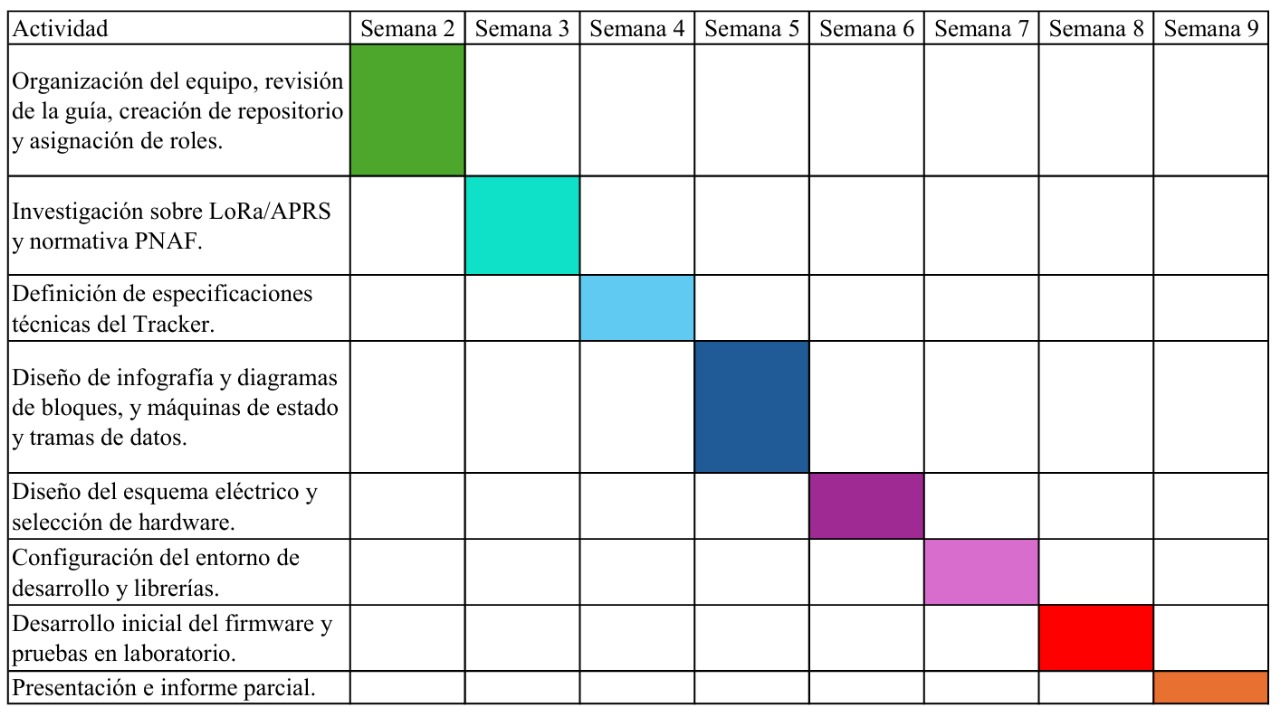
\includegraphics[width=1\linewidth]{fig/Gantt-1.jpeg}
    \caption{Primera parte cronograma}
    \label{fig:gantt1}
\end{figure}

\begin{figure}[htbp]
    \centering
    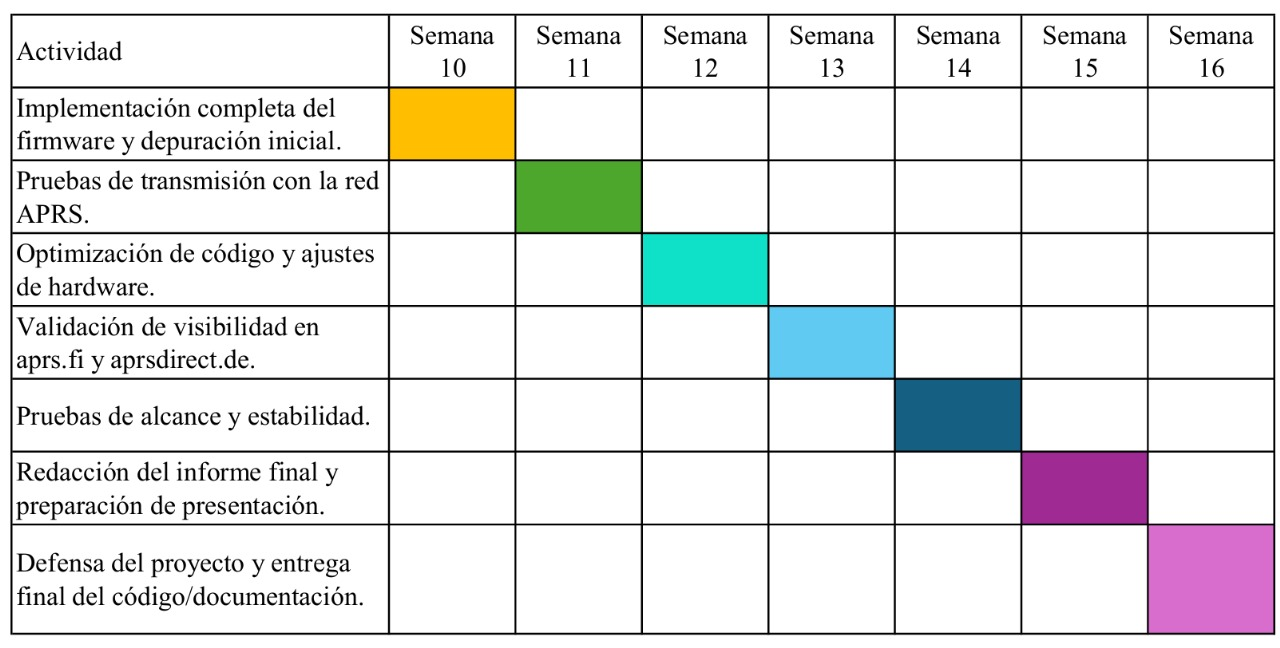
\includegraphics[width=1\linewidth]{fig/Gantt-2.jpeg}
    \caption{Segunda parte cronograma}
    \label{fig:gantt1}
\end{figure}






% Can use something like this to put references on a page
% by themselves when using endfloat and the captionsoff option.
\ifCLASSOPTIONcaptionsoff
  \newpage
\fi



% trigger a \newpage just before the given reference
% number - used to balance the columns on the last page
% adjust value as needed - may need to be readjusted if
% the document is modified later
%\IEEEtriggeratref{8}
% The "triggered" command can be changed if desired:
%\IEEEtriggercmd{\enlargethispage{-5in}}

% references section

% can use a bibliography generated by BibTeX as a .bbl file
% BibTeX documentation can be easily obtained at:
% http://mirror.ctan.org/biblio/bibtex/contrib/doc/
% The IEEEtran BibTeX style support page is at:
% http://www.michaelshell.org/tex/ieeetran/bibtex/
%\bibliographystyle{IEEEtran}
% argument is your BibTeX string definitions and bibliography database(s)
%\bibliography{IEEEabrv,../bib/paper}
%
% <OR> manually copy in the resultant .bbl file
% set second argument of \begin to the number of references
% (used to reserve space for the reference number labels box)

\newpage







% that's all folks
\end{document}


